\nonstopmode

\documentclass[final,letterpaper,12pt]{article}

\usepackage[round, sort]{natbib}

\usepackage[pdftex]{graphicx}
\graphicspath{{Figures/}}

\usepackage{amsmath}

\usepackage{mathtools}

\usepackage{hyperref}

\usepackage{subcaption}

\usepackage{attachfile}

\title{Manual of the \texttt{MATLAB} pipeline for the analysis of genomic time course data from the \textit{Gene Expression Omnibus} (Version 1.53)}

%\author{Juan Camilo Ram\'{i}rez}

\date{\today}

\begin{document}

\maketitle

\tableofcontents

\listoffigures

\listoftables

\section{The Pipeline for Dynamic Gene Expression Data}
\label{section:pipeline}
\par The \textit{Pipeline for Dynamic Gene Expression Data}, also referred to as \texttt{Pipeline4DGEData}, is the implementation of the pipeline proposed by \cite{Carey2017}. It is written in \texttt{MATLAB} (R2016a). The tool is designed to analyze time course data from the \textit{Gene Expression Omnibus} (GEO) in order to discover gene regulatory networks from high-throughput data.

\par Section~\ref{section:theory_and_terminology} provides a very brief summary of the theoretical concepts involved in the usage of \texttt{Pipeline4DGEData}. However, the reader is strongly encouraged to refer to the \href{https://www.ncbi.nlm.nih.gov/geo/}{GEO documentation} and the work of \cite{Carey2017} for full details. Section~\ref{section:Installation} provides installation instructions and Section~\ref{section:daExample} illustrates the usage of \texttt{Pipeline4DGEData}.  The example presented in the latter should be used as basis for other analyses to be performed by the reader.

\section{Theoretical basis and terminology}
\label{section:theory_and_terminology}

\subsection{The \textit{Gene Expression Omnibus (GEO)}}

\par The \textit{Gene Expression Omnibus} (GEO)\footnote{\url{https://www.ncbi.nlm.nih.gov/geo/}} is a public repository administered by the \textit{National Center for Biotechnology Information} (NCBI)\footnote{\url{https://www.ncbi.nlm.nih.gov}} for the storage of high throughput data. The GEO stores microarray data in MIAME compliant formats and makes it publicly available. The data is organized into series, samples and platforms.

\subsection{GEO Series}

\par A data series is a set of related samples. It may also provide information of the investigation associated to the contained samples. The GEO identifies each series by an accession number with the prefix `GSE'. For example, series \href{https://www.ncbi.nlm.nih.gov/geo/query/acc.cgi?acc=GSE59015}{\texttt{GSE59015}}.

\subsection{GEO Samples}

\par The data obtained from an experimental sample. It also describes how the experiment was conducted and how the data was handled or manipulated. The GEO identifies each sample by an accession number with the prefix `GSM'. For example, samples \href{https://www.ncbi.nlm.nih.gov/geo/query/acc.cgi?acc=GSM1424445}{\texttt{GSM1424445}} and \href{https://www.ncbi.nlm.nih.gov/geo/query/acc.cgi?acc=GSM1424453}{\texttt{GSM1424453}}, which are associated to series \href{https://www.ncbi.nlm.nih.gov/geo/query/acc.cgi?acc=GSE59015}{\texttt{GSE59015}}.

\subsection{GEO Platforms}

\par A description of the microarray used to collect a sample. The GEO identifies each platform by an accession number with the prefix `GPL'. For example, platform \href{https://www.ncbi.nlm.nih.gov/geo/query/acc.cgi?acc=GPL17880}{\texttt{GPL17880}}, which is associated to the samples in series  \href{https://www.ncbi.nlm.nih.gov/geo/query/acc.cgi?acc=GSE59015}{\texttt{GSE59015}}.

\subsection{Experimental conditions}
\label{subsection:expconds}

\par An experimental condition is the set of time-independent characteristics or parameters of a sample and/or the circumstances in which it was taken. Usually the main characteristic differentiating a condition from a related one is a stimulus (or lack of), which normally consists of a treatment of viral infection. Depending on the study, other characteristics may be present. These may include, the subject’s gender or cell type used, for instance. The experimental condition excludes the time point, if any.

\par In series \href{https://www.ncbi.nlm.nih.gov/geo/query/acc.cgi?acc=GSE59015}{\texttt{GSE59015}} there are two experimental conditions, namely \texttt{Wildtype} and \texttt{D10}, each one comprising eight samples.

\subsection{Study}

\par A study is a set of samples that refer to a common domain of experimental conditions. A common domain of experimental conditions may consist of, for instance, the presence of a stimulus (treatment or viral infection) and the absence of it. In most cases, the series and study coincide. In these cases, all the samples contained in the series belong to the same study. However, it is possible that the GEO stores series that encompass samples from varying domains. In these cases, the samples contained in the series are grouped into different studies.


\subsection{Experimental macroconditions}

\subsection{Replicates}
\label{subsection:replicates_1}
\par Replicates can be \emph{biological} or \emph{technical}.\footnote{\href{https://honglangwang.wordpress.com/2012/04/24/【bio-glossary】biological-replicates-vs-technical-replicates/}{Biological Replicates vs Technical Replicates}.}

\subsection{Genes' between-replicate noise}
\label{subsection:replicates}
\par Genes may exhibit variation across replicates from the same condition. This variation, referred to as the \emph{gene's between-replicate noise} and denoted by $\delta$, is measured for each gene as follows. Let $x^s_{i,t}$ be the expression level of replicate $s$'s $i$-th gene at time $t$ and let $S$ be the total number of replicates. Let $\sigma_{i,t}$ be the standard deviation of the expression level of the $i$-th gene at time $t$ across the $S$ replicates. The gene $i$'s between-replicate noise, denoted by $\delta_i$,\footnote{Another possibility is to define $\delta_i$ in terms of the coefficient of variation instead of the standard deviation. In other words, the between-replicate noise could be defined as $\delta_i = \frac{1}{T} \sum_{t \in t_1}^{t_T} \frac{\sigma_{i,t}}{\mu_{i,t}}$, where $\mu_{i,t}$ is the mean of the expression level of the $i$-th gene at time $t$ across the $S$ replicates. However, this measure is unreliable given that expression levels are interval scale measures and the coefficient of variation is reliable only in ratio scale measures.} is given by

\begin{equation}
\label{equation:between_replicate_noise}
\delta_i = \frac{1}{T} \sum_{t \in t_1}^{t_T} \sigma_{i,t}.
\end{equation}

\par Section~\ref{section:between_replicate_noise_m} introduces the \texttt{MATLAB} function provided for the calculation of the genes' between-replicate noise from a group of replicates.

\section{Installation of \texttt{Pipeline4DGEData}}
\label{section:Installation}

\par The system requirements of \texttt{Pipeline4DGEData} are listed below.

\begin{itemize}

\item \texttt{MATLAB} R2016a or newer.

\end{itemize}

\par The sources of \texttt{Pipeline4DGEData} are available on its official \href{https://github.com/j142857z/Pipeline4DGEData}{\texttt{GitHub} repository}. The latest version is always availabe for download from \href{https://github.com/j142857z/Pipeline4DGEData/archive/master.zip}{here} as a compressed folder. Once downloaded, this folder must be decompressed. By default, the decompressed folder is named \texttt{Pipeline4DGEData-master/}. In this manual it will be assumed that this folder has been renamed \texttt{Pipeline4DGEData/} and so it will be referred to as such throughout this document. This folder is the home directory of \texttt{Pipeline4DGEData}.\footnote{Care should be taken in order not to confuse \texttt{Pipeline4DGEData} (the tool) and \texttt{Pipeline4DGEData/} (the home folder of the tool).} User-defined input for new analyses to be run must be provided in subfolder \texttt{Input} (details in Section~\ref{section:input_files}) and the program returns the results in subfolder \texttt{Output} (details in Section~\ref{section:pipelineoutput}).

\par \texttt{Pipeline4DGEData} uses the \textit{Functional Data Analysis for \texttt{MATLAB}} library, which is available from its official \href{http://www.psych.mcgill.ca/misc/fda/}{site online}. The library can be downloaded from this \href{http://www.psych.mcgill.ca/misc/fda/downloads/FDAfuns/Matlab/fdaMatlab.zip}{direct link} as a compressed folder. Once downloaded, the decompressed folder (named \texttt{fdaM/}) must be copied to \texttt{Pipeline4DGEData/}. That is to say, all the sources of the library must be in path \texttt{Pipeline4DGEData/fdaM/}. After this, attached file \textattachfile[mimetype=text/html,color=0 0 0.5]{mean_grouped.m}{\texttt{mean\_grouped.m}}  must be copied into \texttt{Pipeline4DGEData/fdaM/@fd/}.

\par \texttt{Pipeline4DGEData} also requires the \textit{\texttt{SBEToolbox} (A Matlab Toolbox for Biological Network Analysis)} library \citep{konganti2013sbetoolbox} (Version \texttt{1.3.3} or later). This library is available from its official \href{https://github.com/biocoder/SBEToolbox/releases}{\texttt{GitHub} repository}. It can be downloaded from this \href{https://github.com/biocoder/SBEToolbox/archive/v1.3.3.zip}{direct link} as a compressed folder. Once downloaded, the decompressed folder (named \texttt{SBEToolbox-1.3.3/}) must be copied to \texttt{Pipeline4DGEData/}. That is to say, all the sources of the library must be in path \texttt{Pipeline4DGEData/SBEToolbox-1.3.3/}.

\par Once all the above is done, \texttt{Pipeline4DGEData} will be ready for use. Details in Section~\ref{section:daExample}.

\section{Usage of \texttt{Pipeline4DGEData}}
\label{section:daExample}

\par This section shows how to use \texttt{Pipeline4DGEData} for the analysis of a set of experimental conditions by illustrating its usage on GEO series \href{https://www.ncbi.nlm.nih.gov/geo/query/acc.cgi?acc=GSE59015}{\texttt{GSE59015}}. Application of \texttt{Pipeline4DGEData} to any other GEO series should be analogous. It is assumed here that has been installed as described in Section~\ref{section:Installation}.

\par GEO series \href{https://www.ncbi.nlm.nih.gov/geo/query/acc.cgi?acc=GSE59015}{\texttt{GSE59015}} refers to a study about the resistance of \textit{Plasmodium falciparum} (\textit{i.e.}, the malaria parasite) to antimalarial drugs for the design of new medications. Two experimental conditions (Section~\ref{subsection:expconds} provides an introduction to experimental conditions) are considered: \texttt{Wildtype} and \texttt{D10}. The latter refers to \textit{P. falciparum} cells that have been exposed to a medication and the former refers to a cells that haven't been exposed to any stimulus and thus serves as the control group. The list of samples is shown in Figure~\ref{fig:GSE59015samples}.

\begin{figure}
	\centering
	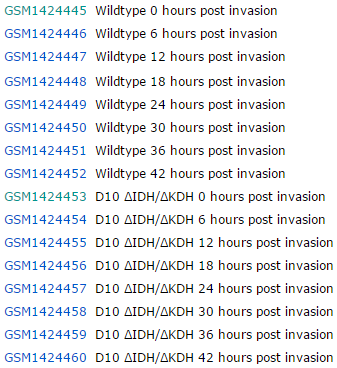
\includegraphics[width=0.5\textwidth]{GSE59015samples}
	\caption{Samples associated to series \texttt{GSE59015}.}
	\label{fig:GSE59015samples}
\end{figure}

\par The following checklist provides the information that is required for running a pipeline analysis. This information should be compiled before starting \texttt{Pipeline4DGEData}.

\begin{enumerate}

\item The accession number of the GEO series.

\begin{itemize}

\item In this example, this number is \texttt{GSE59015}.

\end{itemize}


\item The experimental conditions on which the analysis is to be performed and their corresponding GEO samples. And identifying name should be chosen in advance for each condition.

\begin{itemize}

\item In this example, the conditions' names and their samples are as follows.

\begin{itemize}

\item Condition \texttt{Wildtype} comprising samples \texttt{GSM1424445} through \texttt{GSM1424452}, as shown in Figure~\ref{fig:GSE59015samples}.

\item Condition \texttt{D10} comprising samples \texttt{GSM1424453} through \texttt{GSM1424460}, as shown in Figure~\ref{fig:GSE59015samples}.

\end{itemize}
\end{itemize}
\item The condition files for the conditions on which the analysis is to be performed  (Section~\ref{section:condition_files} provides an introduction to condition files). These files must be located in folder \texttt{Input} and named as specified in Section~\ref{section:input_files}.

\begin{itemize}

\item In this example, the files for the two conditions must be as shown in Figure~\ref{fig:condfilesexample}.
\end{itemize}

\item The accession number of the GEO platform associated to the GEO series.

\begin{itemize}

\item  In this example, this number is \texttt{GPL17880}.
\end{itemize}
\item The index of the column in the GPL record where the gene names are stored.

\begin{itemize}

\item In this example, this index is $7$, as shown in Figure~\ref{fig:GPLexample}.

\end{itemize}
\end{enumerate}


\par Once the above is ready, the analysis can be started by running \texttt{pipeline} from the \texttt{MATLAB} console, as shown in Figure~\ref{fig:pipeline_ex1}. The program will then prompt the user to enter the index of the column in the GPL record where the gene names are located (Item 5 in the checklist above). In this example, this index is $7$ and must be entered as shown in Figure~\ref{fig:pipeline_ex2}. After this the program will proceed to read and match all the probe ids to the corresponding gene names, informing the user that the process can take some time and notifying the progress as shown in Figure~\ref{fig:pipeline_ex3}. When finished, the program will prompt the user to specify the gene ID type used in the dataset by selecting from a predefined list displayed on the \texttt{MATLAB} console. In this example, the type is \texttt{AGILENT\_ID} and thus $5$ must be entered, as shown in Figure~\ref{fig:pipeline_ex4}. After this, the program will start the analysis for ALL the condition files present in folder \texttt{Input}. In this example, the program starts with condition \texttt{D10} as shown in Figure~\ref{fig:pipeline_ex5}. When the analysis has been completed for all the experimental conditions, the program will confirm that the process has been finished successfully, as shown in Figure~\ref{fig:pipeline_ex6}. The results are output to folder \texttt{Output} and organized as explained in Section~\ref{section:pipelineoutput}.

\begin{figure}
	\centering
	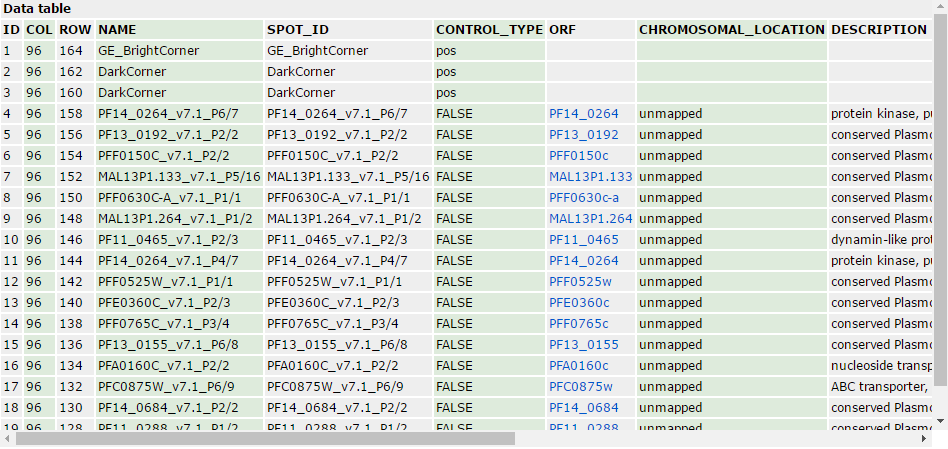
\includegraphics[width=0.95\textwidth]{GPLexample}
	\caption{Table of platform \href{https://www.ncbi.nlm.nih.gov/geo/query/acc.cgi?acc=GPL17880}{\texttt{GPL17880}} showing that the gene names are stored in the $7$-th column (titled \texttt{`ORF'}).}
	\label{fig:GPLexample}
\end{figure}

\begin{figure}
    \centering
    \begin{subfigure}{0.5\textwidth}
        \centering
	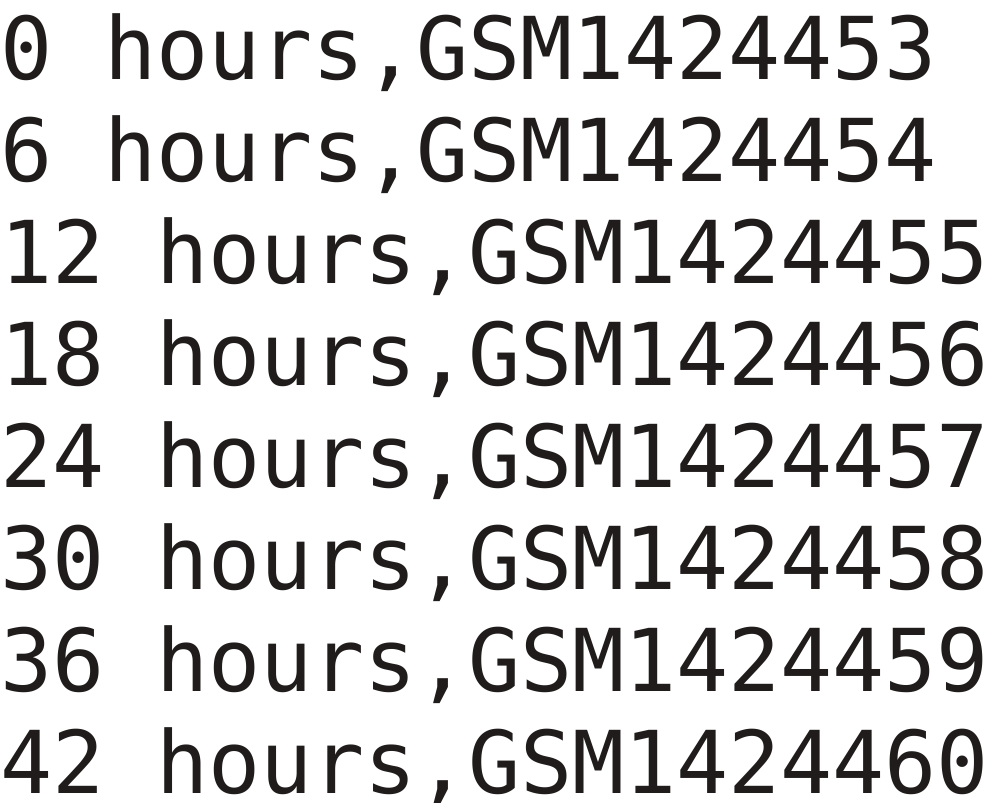
\includegraphics[width=0.45\textwidth]{condfilex1}
        \caption{Condition file for condition \texttt{Wildtype}.}
        \label{fig:condfilex1}
    \end{subfigure} 
    
    \begin{subfigure}{0.5\textwidth}
        \centering
	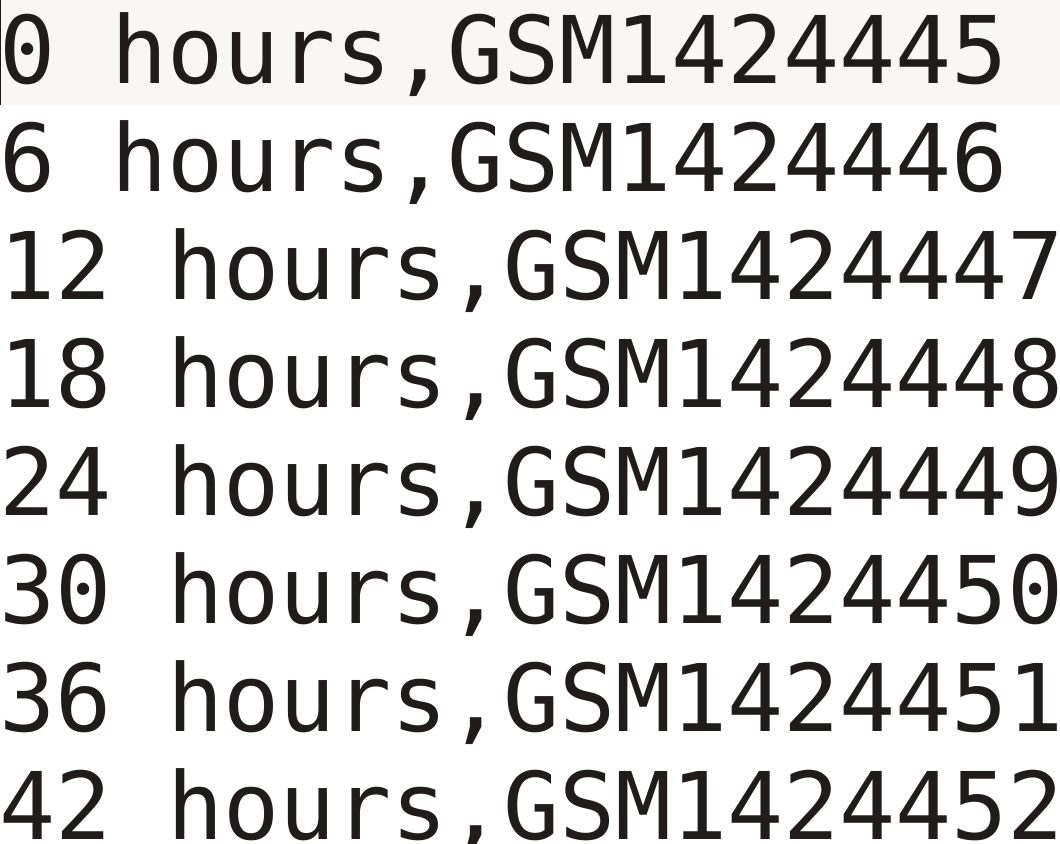
\includegraphics[width=0.45\textwidth]{condfilex2}
        \caption{Condition file for condition \texttt{D10}.}
                \label{fig:condfilex2}
    \end{subfigure}
    \caption{Figure~\ref{fig:condfilex1} shows the contents of the condition file for condition \texttt{Wildtype} and Figure~\ref{fig:condfilex2} shows the contents of the condition file for condition \texttt{D10}.}
    \label{fig:condfilesexample}
\end{figure}



\begin{figure}
	\centering
	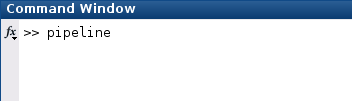
\includegraphics[width=0.95\textwidth]{pipeline_ex1}
	\caption{}
	\label{fig:pipeline_ex1}
\end{figure}

\begin{figure}
	\centering
	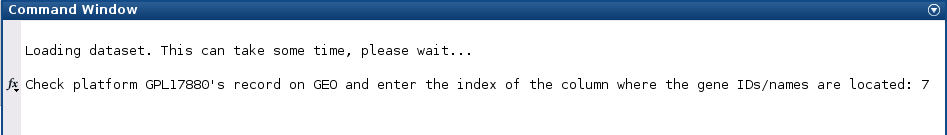
\includegraphics[width=0.95\textwidth]{pipeline_ex2}
	\caption{}
	\label{fig:pipeline_ex2}
\end{figure}

\begin{figure}
	\centering
	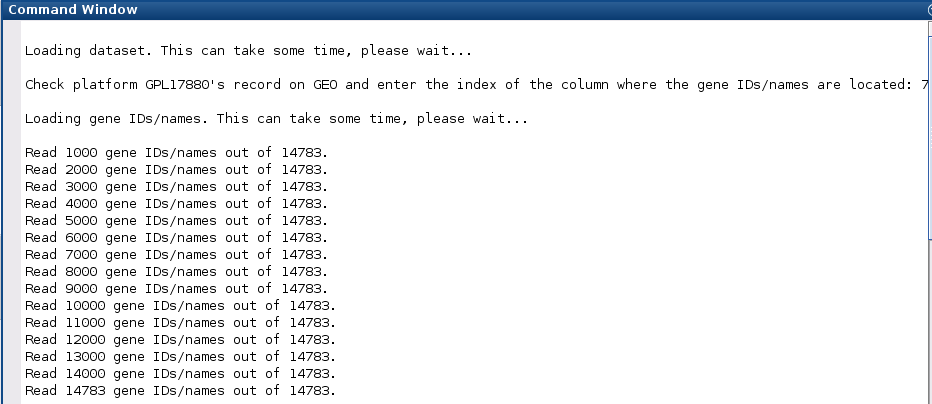
\includegraphics[width=0.95\textwidth]{pipeline_ex3}
	\caption{}
	\label{fig:pipeline_ex3}
\end{figure}

\begin{figure}
	\centering
	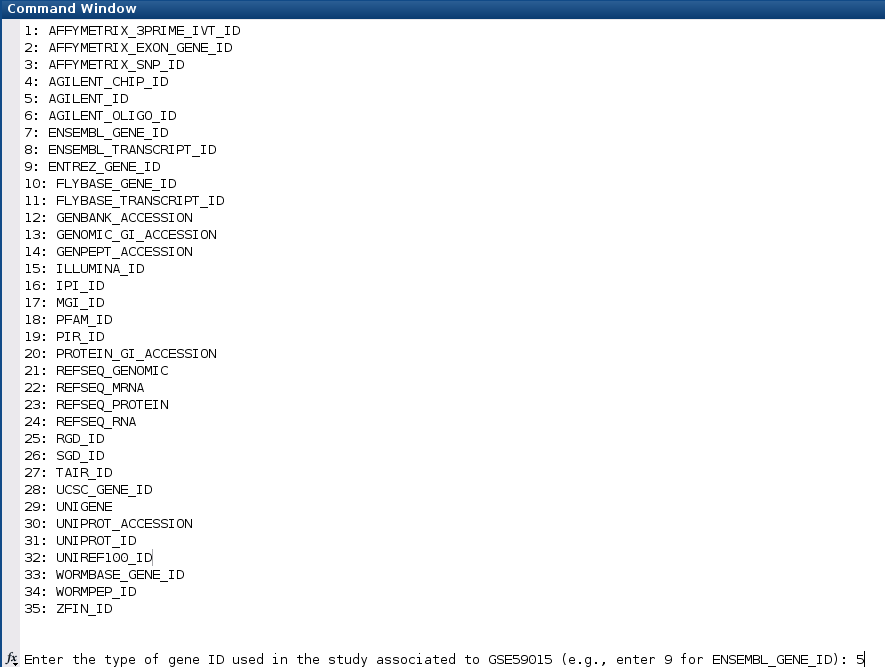
\includegraphics[width=0.95\textwidth]{pipeline_ex4}
	\caption{}
	\label{fig:pipeline_ex4}
\end{figure}


\begin{figure}
	\centering
	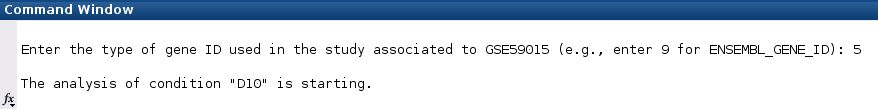
\includegraphics[width=0.95\textwidth]{pipeline_ex5}
	\caption{}
	\label{fig:pipeline_ex5}
\end{figure}


\begin{figure}
	\centering
	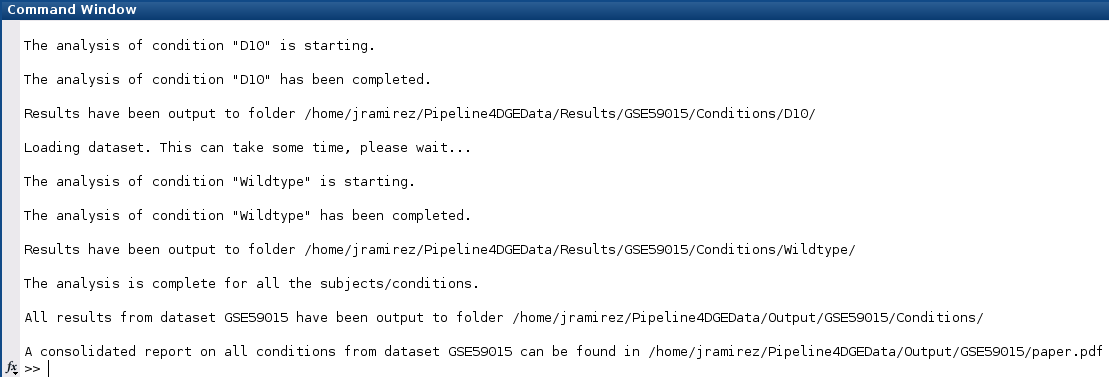
\includegraphics[width=0.95\textwidth]{pipeline_ex6}
	\caption{}
	\label{fig:pipeline_ex6}
\end{figure}







\section{Input files}
\label{section:input_files}

\subsection{Condition files}
\label{section:condition_files}

\par \emph{Condition files} are the input files for the pipeline analysis of one or more experimental conditions (See Section~\ref{subsection:expconds} regarding experimental conditions). The information of each experimental condition must be provided in a text file. One file for each condition. The condition files must be stored in folder \texttt{Input}. Each condition file must be named with the following format: \texttt{[GEO SERIES NUMBER]\_-\_[NAME OF EXPERIMENTAL CONDITION]\_-\_[NUMBER OF TOP DRGs FOR CLUSTERING].txt}.

\par All the samples associated with the experimental condition must be provided along with the time points using the format described as follows. Each line of the file must consist of the time point, including the time unit (e.g., 2 hours), followed by a comma (,) and then followed by the accession number of one sample. For example, the file for condition ``D10'' of \textit{GEO} series \texttt{GSE59015} must be named \texttt{GSE59015\_-\_D10\_-\_3000.csv} and the contents must be as follows.

\begin{center}
\begin{tabular}{ c }

0 hours,GSM1424453 \\
6 hours,GSM1424454 \\
12 hours,GSM1424455 \\
18 hours,GSM1424456 \\
24 hours,GSM1424457 \\
30 hours,GSM1424458 \\
36 hours,GSM1424459 \\
42 hours,GSM1424460 \\

\end{tabular}
\end{center}

\par The condition file can group different replicates that represent the same experimental condition. In this case the pipeline will run one single analysis with the average of all the replicates specified in the file. For example, the file for all the replicates in \textit{GEO} series \texttt{GSE41067} must be named \texttt{GSE41067\_-\_ALL\_-\_10000.csv} and the contents must be as follows.

\begin{center}
\begin{tabular}{ c }

0 hours,GSM1008154,GSM1008162,GSM1008170 \\
1 hours,GSM1008155,GSM1008163,GSM1008171 \\
2 hours,GSM1008156,GSM1008164,GSM1008172 \\
4 hours,GSM1008157,GSM1008165,GSM1008173 \\
6 hours,GSM1008158,GSM1008166,GSM1008174 \\
8 hours,GSM1008159,GSM1008167,GSM1008175 \\
10 hours,GSM1008160,GSM1008168,GSM1008176 \\
12 hours,GSM1008161,GSM1008169,GSM1008177 \\


\end{tabular}
\end{center}

\par The condition files can be written manually, following strictly the format described above. Optionally, this task can be carried out more easily by using script \texttt{create\_input\_files.m}. In order to do this, \texttt{create\_input\_files.m} must be run and the instructions provided thereafter by the program must be followed. More details in Section~\ref{section:user_functions}.

\subsection{Macrocondition files}
\label{subsection:macrocondition}

\par The conditions comprising the macrocondition must be provided in a text file that must be located in folder \texttt{Input}. This file must be named using the following format: \texttt{[GEO SERIES NUMBER]\_-\_[NAME OF MACRO CONDITION].txt}. For example, the following are the contents of a macrocondition of five H3N1 subjects from \texttt{GSE52428}.

\begin{center}
\begin{tabular}{ c }

H3N1\_001 \\
H3N1\_002 \\
H3N1\_003 \\
H3N1\_004 \\
H3N1\_005 \\

\end{tabular}
\end{center}


\par This file can be constructed manually, or with BASH script \texttt{prepare\_input.sh}. This option requires running the script with the following syntax.

\texttt{./prepare\_input.sh [GEO SERIES] [NAME OF MACRO CONDITION].txt}

\par Example

\texttt{./prepare\_input.sh GSE52428 H1N1.txt}

\par The above will read ALL the conditions whose analyses have been completed for the GEO series indicated and write the file with the format described earlier.

\section{Output of results}
\label{section:pipelineoutput}

\par \texttt{Pipeline4DGEData} outputs all of its results to subfolder \texttt{Output}. Each pipeline analysis is carried out on an experimental condition and results from several conditions are grouped in folder by the accesion number of the associated GEO series.

\section{Guided creation of condition files}
\label{section:user_functions}

\par The (experimental) condition files for the pipeline analysis can be created manually with the format described in Section~\ref{section:condition_files} on page \pageref{section:condition_files} or with the help of script \texttt{create\_input\_files.m}. In order to do the latter, the command \texttt{create\_input\_files} must be executed on the \texttt{MATLAB} console from the pipeline directory.

\par Prior to running the pipeline analysis for the two conditions (Subsection~\ref{section:condition_files} provides an introduction to conditions files), the corresponding condition files must be created. In order to do this, \texttt{MATLAB} must be started \underline{inside} folder \texttt{Pipeline4DGEData/} and in the console the command \texttt{create\_input\_files} must be called, as shown in Figure~\ref{fig:create_input_files1} and then pressing \texttt{Enter}.

\begin{figure}
	\centering
	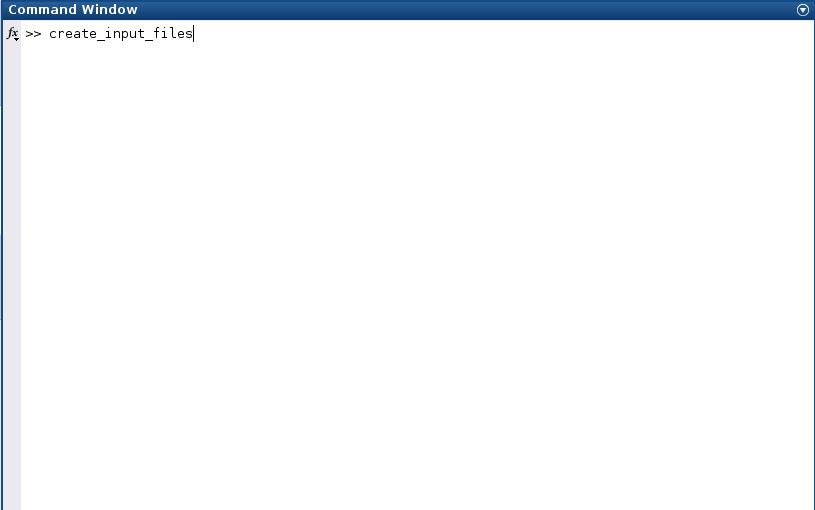
\includegraphics[width=0.65\textwidth]{create_input_files1}
	\caption{Calling \texttt{create\_input\_files} to create condition files.}
	\label{fig:create_input_files1}
\end{figure}

\par The program will then request the accession number of the GEO series on which the analysis is to be performed. This information must be entered as single quotes ('), as shown in  Figure~\ref{fig:create_input_files2}. In this example, the accession number entered is \texttt{GSE59015}.

\begin{figure}
	\centering
	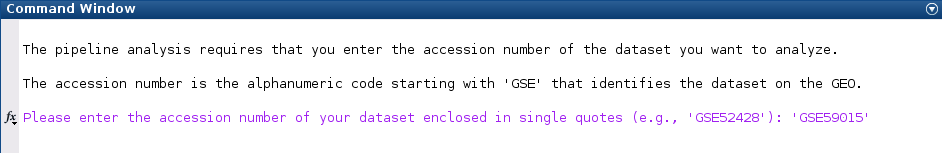
\includegraphics[width=0.95\textwidth]{create_input_files2}
	\caption{Entering the accession number for the creation of the condition files.}
	\label{fig:create_input_files2}
\end{figure}

\begin{figure}
	\centering
	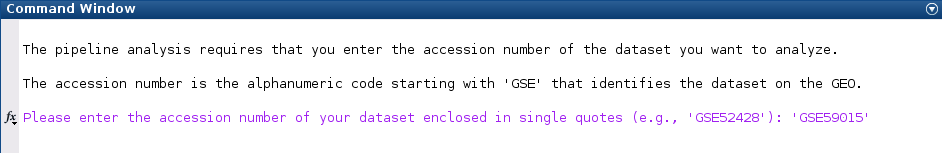
\includegraphics[width=0.95\textwidth]{create_input_files2}
	\caption{Entering the accession number for the creation of the condition files.}
	\label{fig:create_input_files2}
\end{figure}

\par After hitting \texttt{Enter}, the program will read the series data from the GEO and will request the index of the column where the gene names are located in the platform record.

\section{\texttt{compare.m}}

\par A comparison can be performed between each pair of experimental conditions from a GEO series. This comparison includes an examination of how one gene behaves under one condition against the other and what modules in one condition match closest in expression pattern another module from the other condition.

\par This comparison can be performed once the regular pipeline analysis is completed for the given GEO series and results are stored in folder \texttt{Output}. The comparison can be launched by executing \texttt{compare.m} whose input is a macrocondition file. See Subsection~\ref{subsection:macrocondition}.

\par An important requirement is that all the conditions to be compared (\textit{i.e.}, those listed in the macrocondition file) have the same number of time points. Some series in the GEO include conditions with different numbers of time points. If a comparison is needed between these, then the pipeline analysis must be done on these including the samples where the to-be-compared conditions agree on the time points.

\section{\texttt{measure\_fit\_of\_replicates.m}}
\label{section:between_replicate_noise_m}

\par This is a script that calculates the between-replicate noise for all genes across a number of replicates, as shown in Subsection~\ref{subsection:replicates}. Its input is a macrocondition file, as defined in Subsection~\ref{subsection:macrocondition}. Results will be output in folder \texttt{Pipeline\_HOME/Output/[GSE Series]/Comparison\_of\_replicates/[Macrocondition]/}.

\par This folder contains a file named \texttt{[Macrocondition]\_noise\_per\_gene\_ALL\_GENES.csv}. Each line of this file corresponds to a probe in the GSE matrix and contains three values separated by commas (,). The first field is the probe ID, the second is the gene name, and the third is the gene's between-replicate noise. The probes are listed in this file in the same order they appear in the GSE matrix. A secondary file, named \texttt{[Macrocondition]\_noise\_per\_gene\_ALL\_GENES\_SORTED\_BY\_NOISE.csv}, provides the same information with the probes listed by their between-replicate noise in decreasing order. That is to say, probes that appear on top are the ones whose expression is most consistent across the probes provided in the macrocondition file whereas those at the bottom are the ones exhibiting the most discrepancy in expression across these replicates.


\section{Output of the pipeline}
\label{section:pipeline_output}

\par All results are output to folder \texttt{Output}. Results are grouped by the \textit{GEO} series' accession number and by the name of the experimental condition, as illustrated in Figure~\ref{fig:results_hierarchy_1}.


\begin{figure}
	\centering
	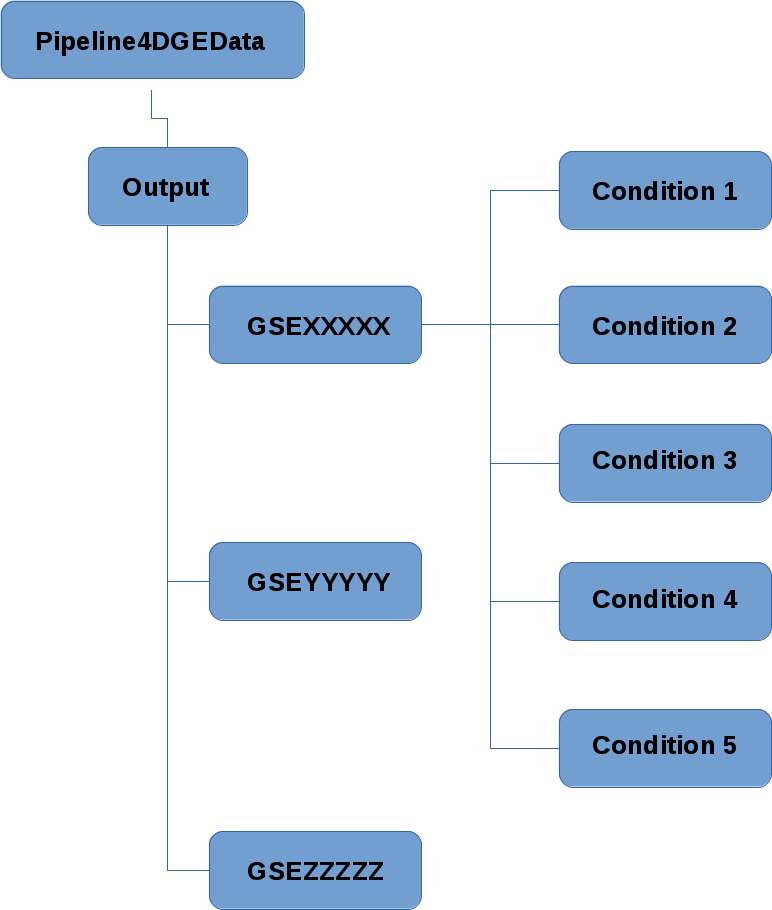
\includegraphics[width=\textwidth]{FolderHierarchy1}
	\caption{Folder hierarchy of results.}
	\label{fig:results_hierarchy_1}
\end{figure}


\section{Simulation of time course data}
\label{section:simulation}

\par The robustness of the pipeline process can be validated by simulating gene expression data and verifying if the pipeline returns the same model the simulated data originate from. More specifically, expression data can be simulated from given a GRN and set of GRMs and given as input to the pipeline in order to verify that the algorithm approximates the original GRN and GRMs. In order to achieve this, two types of the gene expression curves need to be generated: those from DRGs and those from non-DRGs. First, the expression curves of the DRGs are simulated from the mean curves of the GRMs as follows. Let $K$ be the matrix representing the expression of one gene response module composed of $n$ genes over $t$ time points, given by

\begin{equation*}
K = 
 \begin{pmatrix}
  X_{1,1} & X_{1,2} & \cdots & X_{1,t} \\
  X_{2,1} & X_{2,2} & \cdots & X_{2,t} \\
  \vdots  & \vdots  & \ddots & \vdots  \\
  X_{n,1} & X_{n,2} & \cdots & X_{n,t} 
 \end{pmatrix}.
\end{equation*}


\par Also let $M$ be the tuple of per-column means of $K$, given by

\begin{equation*}
M = 
 \begin{pmatrix}
  \mu_{1} & \mu_{2} & \cdots & \mu_{t}
 \end{pmatrix},
\end{equation*}

and let $S$ be the per-column standard deviation of $K$, given by

\begin{equation*}
S = 
 \begin{pmatrix}
  \sigma_{1} & \sigma_{2} & \cdots & \sigma_{t}
 \end{pmatrix}.
\end{equation*}

Then $n$ simulated curves are obtained where the $i$-th element is a normal deviate of $\mu_{i}$ with standard deviation $\sigma_{i}$. This process is repeated for all the GRMs until obtaining the simulated expression curves of all the DRGs. Thereafter, the non-DRG curves are simulated as normal deviates of the per-time point means of all the DRG curves, with standard deviation $1.0$. The simulated DRG and non-DRG expression curves can then be passed as arguments to the pipeline and see if the GRMs and GRN obtained approximate the originals.

\par The procedure described above is performed by script \texttt{run\_simulation.m}, which reads the results of a previously-completed analysis from folder \texttt{Output}, constructs the simulated data and runs the pipeline in folder \texttt{Output/[Condition]\_simulated}, where \texttt{[Condition]} is the name of the original experimental condition.

\bibliographystyle{myapalike}
\bibliography{bibliography}
\end{document}

